\documentclass[10pt]{beamer}
\usetheme[
%%% option passed to the outer theme
%    progressstyle=fixedCircCnt,   % fixedCircCnt, movingCircCnt (moving is deault)
  ]{Feather}
\usepackage[utf8]{inputenc}
\usepackage{tikz}
% If you want to change the colors of the various elements in the theme, edit and uncomment the following lines

% Change the bar colors:
%\setbeamercolor{Feather}{fg=red!20,bg=red}

% Change the color of the structural elements:
%\setbeamercolor{structure}{fg=red}

% Change the frame title text color:
%\setbeamercolor{frametitle}{fg=blue}

% Change the normal text color background:
%\setbeamercolor{normal text}{fg=black,bg=gray!10}

%-------------------------------------------------------
% INCLUDE PACKAGES
%-------------------------------------------------------

\usepackage[utf8]{inputenc}
\usepackage[english]{babel}
\usepackage[T1]{fontenc}
\usepackage{helvet}

%-------------------------------------------------------
% DEFFINING AND REDEFINING COMMANDS
%-------------------------------------------------------

% colored hyperlinks
\newcommand{\chref}[2]{
  \href{#1}{{\usebeamercolor[bg]{Feather}#2}}
}

%-------------------------------------------------------
% INFORMATION IN THE TITLE PAGE
%-------------------------------------------------------

\title[] % [] is optional - is placed on the bottom of the sidebar on every slide
{ % is placed on the title page
      \textbf{MATRIX PROJECT}
}

\subtitle[MATRIX PROJECT]
{
      \textbf{ASDSAD}
}

\author[SHRUTI \& SHRESHTA]
{      SHRUTI \& SHRESHTA \\
      {}
}

\institute[]
{
      Universidad Manuela Beltrán 
      Biomateriales
  
  %there must be an empty line above this line - otherwise some unwanted space is added between the university and the country (I do not know why;( )
}

\date{\today}

%-------------------------------------------------------
% THE BODY OF THE PRESENTATION
%-------------------------------------------------------

\begin{document}



%-------------------------------------------------------
% THE TITLEPAGE
%-------------------------------------------------------

{\1% % this is the name of the PDF file for the background}



\begin{frame}{\bf MATRIX PROJECT}{}

{\bf INTRODUCTION TO AI AND ML }                 
\newline

EE1390
\newline

\newline
 {\bullet C.SHRUTI}
\newline
    \bullet SHRESHTA.T
\end{frame}

%-------------------------------------------------------
\section{Introduction}
%-------------------------------------------------------
\subsection{Arterias,Venas y vasos Linfáticos}
\begin{frame}{QUESTION IN GEOMETRIC FORM     }

    Que. Find the tangent to the circle, at the point (1,-1)
    whose centre is the point of intersection of the straight lines

    \begin{equation}
        2x+y=3
    \end{equation}
    ,
    \begin{equation}
        x-y=1
    \end{equation}
\end{frame}
\begin{frame}{QUESTION IN MATRIX FORM}

Que. Find the tangent to the circle, at the point 
\[
\begin{bmatrix}
1\\
-1
\end{bmatrix}

\]
,whose centre is the point of intersection of the straight lines

\[
\begin{bmatrix}
2 & 1
\end{bmatrix}
X=3
\]
\[
\begin{bmatrix}
1 & -1
\end{bmatrix}
X=1
\]

 
\end{frame}
\begin{frame}{SOLUTION}
%-------------------------------------------------------

 
    \[
\begin{bmatrix}
2 & 1
\end{bmatrix}
\begin{bmatrix}
x\\
y
\end{bmatrix}
=3

\]

 \[
\begin{bmatrix}
1 & -1
\end{bmatrix}
\begin{bmatrix}
x\\
y
\end{bmatrix}
=1

\]
 \[
\begin{bmatrix}
2 & 1\\
1 & -1
\end{bmatrix}
\begin{bmatrix}
x\\
y
\end{bmatrix}
=
\begin{bmatrix}
3\\
1
\end{bmatrix}

\]
 \[
\begin{bmatrix}
x\\
y
\end{bmatrix}
=
\begin{bmatrix}
-1 & -1\\
-1 & 2

\end{bmatrix}
\begin{bmatrix}
3\\
1
\end{bmatrix}

\]

\begin{equation}
x=4/3=a 
\end{equation}
\begin{equation}
y=1/3=b 
\end{equation}

\end{frame}
\begin{frame}{SOLUTION}
Let 'O' be the center of the circle and 'P' be the point at which tangent is to be drawn,
\begin{equation}
O=
\begin{bmatrix}
a\\
b
\end{bmatrix}
=
\begin{bmatrix}
4/3\\
1/3
\end{bmatrix}
\end{equation}   
\begin{equation}
P=
\begin{bmatrix}
1\\
-1
\end{bmatrix}
\end{equation}  
\begin{equation}
OP=r=
|| O - P ||
\end{equation}  
\begin{equation}
OP^2=r^2=(a-1)^2+(b+1)^2
\end{equation}  
\begin{equation}
r^2=(1/3)^2+(4/3)^2=17/9
\end{equation}  

\end{frame}
\begin{frame}{SOLUTION}
Equation of circle:
\begin{equation}
XX^T+
\begin{bmatrix}
-8/3\\
-2/3
\end{bmatrix}
X=0
\end{equation}
Parametric form of circle:

\begin{equation}
\begin{bmatrix}
x\\
y
\end{bmatrix}
=
\begin{bmatrix}
4/3\\
1/3
\end{bmatrix}
+r
\begin{bmatrix}
cos(\theta)\\
sin(\theta)
\end{bmatrix}
\end{equation}    
0< \theta <2\pi

Equation of circle:
\begin{equation}
x^2+y^2-8/3x-2/3y=0  
\end{equation}
\end{frame}

\begin{frame}{EQUATION OF TANGENT}
Direction vector of radius = Direction of normal vector of the tangent:
\begin{equation}
OP=r=
\begin{bmatrix}
1/3\\
4/3
\end{bmatrix}
\end{equation}
Equation of tangent;
\begin{equation}
\begin{bmatrix}
1/3 & 4/3 \\
\end{bmatrix}
X=-1
\end{equation}

Hence, equation of tangent is:

\begin{equation}
x+4y+3=0    
\end{equation}
\end{frame}
\begin{frame}{DIRECTION VECTOR OF TANGENT}




Direction vector of tangent = normal of radius vector

\begin{equation}
\begin{bmatrix}
0 & 1\\
-1 & 0
\end{bmatrix}
\begin{bmatrix}
1/3\\
4/3
\end{bmatrix}
=
\begin{bmatrix}
4/3 \\
-1/3
\end{bmatrix}
\end{equation}
    
\end{frame}

\begin{frame}{FIGURE OF SOLUTION}

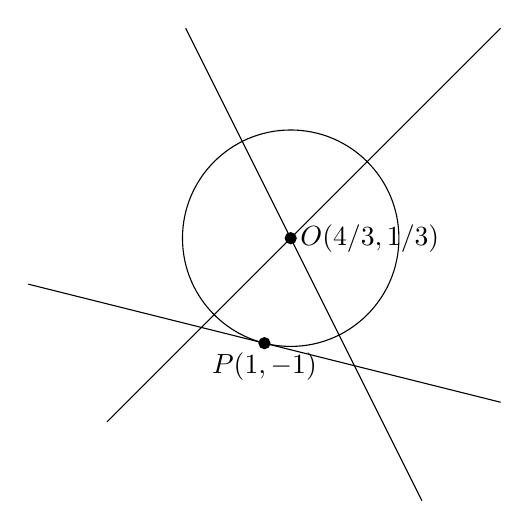
\begin{tikzpicture}
\draw(4/3,1/3) circle(1.37436854cm);

\draw (0,3) -- (3,-3);
\draw (-1,-2) -- (4,3);  
\draw (4,-7/4) -- (-2,-1/4);

\draw (4/3,1/3) circle(2pt)      node[right] {$O(4/3,1/3)$}; ;
\fill (4/3,1/3)  circle[radius=2pt]     ;
\draw(1,-1) circle(2pt)         node[below] {$P(1,-1)$};;
\fill (1,-1)  circle[radius=2pt];

\end{tikzpicture}



\end{frame}
\begin{frame}{FIGURE OF SOLUTION}
\begin{figure}

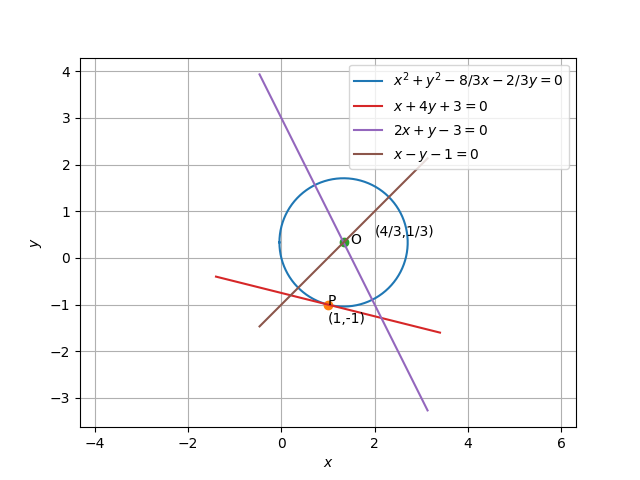
\includegraphics[scale=0.6]{figure.png}
    
\end{figure}
\end{frame}
\end{document}